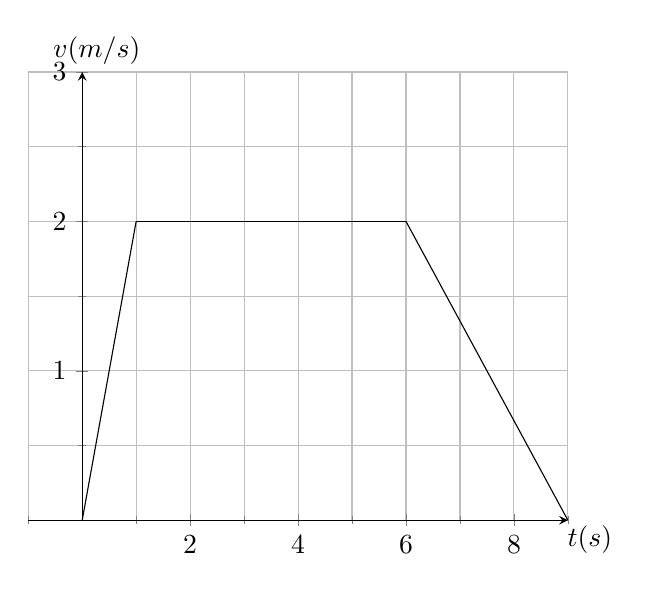
\begin{tikzpicture}
  \begin{axis}[grid=both,%
    %axis x line=center,%
  %axis y line=center,%
    ymin=0,ymax=3,xmax=9,xmin=-1,%
    %xticklabel=\empty,%
    %yticklabel=\empty, %
    minor tick num=1,axis lines = middle,xlabel=$t(\si{s})$,ylabel=$v(\si{m/s})$,label style =
               {at={(ticklabel cs:1.1)}}]
    \addplot [mark=none,domain=0:1] {2*x};
    \addplot [mark=none,domain=1:6] {2};
    \addplot [mark=none,domain=6:9] {6 -2*x/3};
  \end{axis}
  % \draw [very thin, gray] (0,0) grid (12,4);
  % \path(0 ,0)coordinate(A);
  % \path(3 ,2)coordinate(B);
  % \path(10 ,4)coordinate(C);
  % \path(0 ,2)coordinate(ctrl1);
  % \path(2 ,1)coordinate(ctrl2);
  % \path(4 ,3)coordinate(ctrl3);
  % \path(10 ,2)coordinate(ctrl4);
  % \path(10, 6)coordinate(ctrl5);
  % \draw(A)  .. controls(ctrl1)and(ctrl2)  ..  (B) .. controls(ctrl3)and(ctrl4) .. (C);%
  % \UPSTIprofOnly{\draw[->,red,very thick] (B) -- (ctrl3) node[near end, above] {\vVitesse{B}{}{0}};}
  % \draw[red] (B) node{$\bullet$} node[above]{B};
  % \UPSTIprofOnly{\draw[->,blue,very thick] (A) -- (ctrl1) node[near end, below right] {\vVitesse{A}{}{0}};}
  % \draw[blue] (A) node{$\bullet$} node[below]{A};
  % \UPSTIprofOnly{\draw[->,blue,very thick] (C) -- (ctrl5) node[near end, below right] {\vVitesse{C}{}{0}};}
  % \draw[darkspringgreen] (C) node{$\bullet$} node[right]{C};
\end{tikzpicture}
